\subsection{View Models en Reactive UI} 
\label{sec:vm-reactive-ui}

Voor de koppeling tussen views en data gebruiken we speciale ViewModels die een `lifetime' hebben die langer is dan de views die deze modellen gebruiken. Controllers vragen de ViewModels op en geven ze door aan de views. Elke view bind zich vast aan het ViewModel en als een veld van het model verandert, dan updaten de views automatisch. Dit werkt met ReactiveUI~\footnote{\url{http://www.reactiveui.net/}}, een UI framework dat gebruikmaakt van \ac{rx}. Elk veld van de ViewModels stuurt een notificatie naar alle luisterende views als het wordt aangepast. ReactiveUI levert hiervoor zowel het notificatie-systeem als het koppel systeem voor views. Een versimpeld voorbeeld is als volgt:

% public class SpeedViewModel : ReactiveObject {
%   private double _speed = 0;
%   public double Speed { 
%     get { return _speed; }
%     set { RaiseAndSetIfChanged(ref _speed, value); }
%   }
% }

% public class View : UIView, IViewFor<SpeedViewModel> {
%   public View(SpeedViewModel model) {
%     OneWayBind(
%       model, vm => vm.Speed, 
%       view => view.speedLabel.Text, 
%       field => field.ToString("F") + " km/h"
%     );
%   }
% }

% pygmentize -f tex -l csharp -o out.tex in.cs

\begin{Verbatim}[commandchars=\\\{\}]
\PY{k}{public} \PY{k}{class} \PY{n+nc}{SpeedViewModel} \PY{p}{:} \PY{n}{ReactiveObject} \PY{p}{\PYZob{}}
  \PY{k}{private} \PY{k+kt}{double} \PY{n}{\PYZus{}speed} \PY{p}{=} \PY{l+m}{0}\PY{p}{;}
  \PY{k}{public} \PY{k+kt}{double} \PY{n}{Speed} \PY{p}{\PYZob{}}
    \PY{k}{get} \PY{p}{\PYZob{}} \PY{k}{return} \PY{n}{\PYZus{}speed}\PY{p}{;} \PY{p}{\PYZcb{}}
    \PY{k}{set} \PY{p}{\PYZob{}} \PY{n}{RaiseAndSetIfChanged}\PY{p}{(}\PY{k}{ref} \PY{n}{\PYZus{}speed}\PY{p}{,} \PY{k}{value}\PY{p}{)}\PY{p}{;} \PY{p}{\PYZcb{}}
  \PY{p}{\PYZcb{}}
\PY{p}{\PYZcb{}}

\PY{k}{public} \PY{k}{class} \PY{n+nc}{View} \PY{p}{:} \PY{n}{UIView}\PY{p}{,} \PY{n}{IViewFor}\PY{p}{\PYZlt{}}\PY{n}{SpeedViewModel}\PY{p}{\PYZgt{}} \PY{p}{\PYZob{}}
  \PY{k}{public} \PY{n+nf}{View}\PY{p}{(}\PY{n}{SpeedViewModel} \PY{n}{model}\PY{p}{)} \PY{p}{\PYZob{}}
    \PY{n}{OneWayBind}\PY{p}{(}
      \PY{n}{model}\PY{p}{,} \PY{n}{vm} \PY{p}{=}\PY{p}{\PYZgt{}} \PY{n}{vm}\PY{p}{.}\PY{n}{Speed}\PY{p}{,}
      \PY{n}{view} \PY{p}{=}\PY{p}{\PYZgt{}} \PY{n}{view}\PY{p}{.}\PY{n}{speedLabel}\PY{p}{.}\PY{n}{Text}\PY{p}{,}
      \PY{n}{field} \PY{p}{=}\PY{p}{\PYZgt{}} \PY{n}{field}\PY{p}{.}\PY{n}{ToString}\PY{p}{(}\PY{l+s}{\PYZdq{}F\PYZdq{}}\PY{p}{)} \PY{p}{+} \PY{l+s}{\PYZdq{} km/h\PYZdq{}}
    \PY{p}{)}\PY{p}{;}
  \PY{p}{\PYZcb{}}
\PY{p}{\PYZcb{}}
\end{Verbatim}

%\caption{Voorbeeld van ReactiveUI: een ViewModel en View}

Wanneer de controller nu een ViewModel aanpast, of er via SignalR een update binnenkomt, dan wordt de view direct aangepast. 

Naast het updaten van alleenstaande modellen, gebruiken we ook lijsten van modellen. Hiervoor gebruiken we ReactiveList's, uit ReactiveUI, welke notificaties kunnen sturen wanneer er een element wordt toegevoegd of wordt verwijderd uit de lijst. We updaten dan de bestaande tabel en hoeven niet de hele tabel opnieuw te tekenen.

Door gebruik te maken van ReactiveUI wordt het heel simpel om views te maken die `live' zijn en het zorgt er voor dat de code overzichtelijk blijft, omdat het invullen en updaten van de views met dezelfde code gebeurt en deze erg simpel is.

\subsection{Grafische user interface}

De gebruikersinterface van de applicatie staat in principe los van de rest van de applicatie. Hoewel het grootste deel van de code gebruikt kan worden op verschillende platforms, moet de gebruikersinterface voor elk platform apart ontwikkeld worden. Tijdens dit bachelorproject is ervoor gelozen om alleen een specifieke gebruikersinterface te maken voor iPhones. Hiervoor is gekozen omdat het grootste deel van de KNSB-top een iPhone gebruikt. Wanneer zij besluiten dat de applicatie ook daadwerkelijk gebruikt gaat worden, kunnen er nog gebruikersinterfaces gebouwd worden voor andere populaire platforms.

\begin{figure}[h!t]
\centering
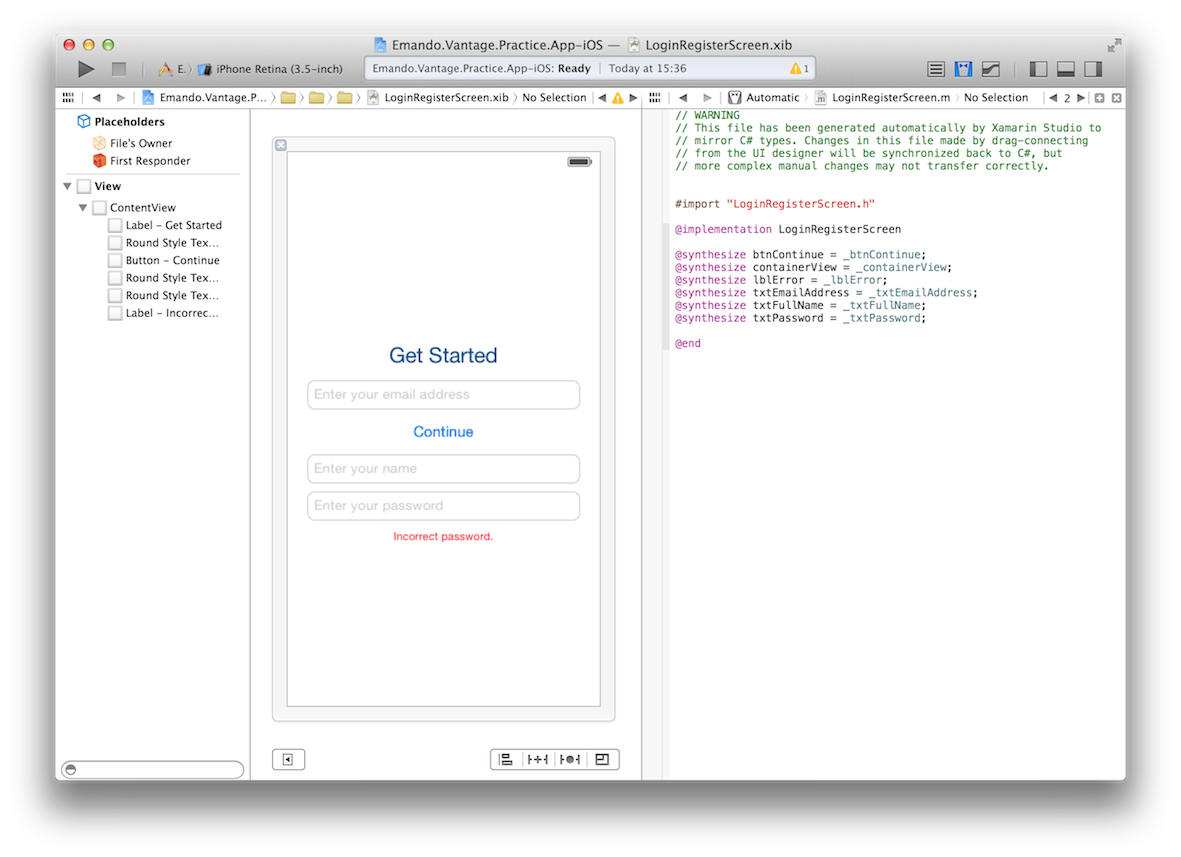
\includegraphics[width=\textwidth]{style/images/screenshots/InterfaceBuilder}
\caption{De XCode Interface Builder}
\label{fig:interface-builder}
\end{figure}

Door het gebruik van Xamarin gaat de implementatie van de iOS user interface iets anders dan met reguliere iOS applicaties. Er kan deels gebruikgemaakt worden van de Interface Builder (figuur~\ref{fig:interface-builder}) die ingebouwd zit in Xcode, de officiële ontwikkelomgeving voor iOS.

Na het opslaan van de gebruikersinterface in Xcode, genereert de Xamarin omgeving automatisch code zoals hieronder weergegeven, waarmee de native interface kan worden aangesloten op C\#.

% [Register ("LoginRegisterScreen")]
% partial class LoginRegisterScreen
% {
%   [Outlet]
%   MonoTouch.UIKit.UIButton btnContinue { get; set; }
%   [Outlet]
%   MonoTouch.UIKit.UILabel lblError { get; set; }
%   [Outlet]
%   MonoTouch.UIKit.UITextField txtEmailAddress { get; set; }

% pygmentize -f tex -l csharp -o out.tex in.cs

\begin{Verbatim}[commandchars=\\\{\}]
\PY{n+na}{[Register (\PYZdq{}LoginRegisterScreen\PYZdq{})]}
\PY{k}{partial} \PY{k}{class} \PY{n+nc}{LoginRegisterScreen}
\PY{p}{\PYZob{}}
\PY{n+na}{  [Outlet]}
  \PY{n}{MonoTouch}\PY{p}{.}\PY{n}{UIKit}\PY{p}{.}\PY{n}{UIButton} \PY{n}{btnContinue} \PY{p}{\PYZob{}} \PY{k}{get}\PY{p}{;} \PY{k}{set}\PY{p}{;} \PY{p}{\PYZcb{}}
\PY{n+na}{  [Outlet]}
  \PY{n}{MonoTouch}\PY{p}{.}\PY{n}{UIKit}\PY{p}{.}\PY{n}{UILabel} \PY{n}{lblError} \PY{p}{\PYZob{}} \PY{k}{get}\PY{p}{;} \PY{k}{set}\PY{p}{;} \PY{p}{\PYZcb{}}
\PY{n+na}{  [Outlet]}
  \PY{n}{MonoTouch}\PY{p}{.}\PY{n}{UIKit}\PY{p}{.}\PY{n}{UITextField} \PY{n}{txtEmailAddress} \PY{p}{\PYZob{}} \PY{k}{get}\PY{p}{;} \PY{k}{set}\PY{p}{;} \PY{p}{\PYZcb{}}
\end{Verbatim}

De gebruikersinterface van de applicatie is in twee lagen gestructureerd. Allereerst zijn er de verschillende tabs waarmee de gebruiker kan wisselen tussen de verschillende contexten: persoonlijk, favorieten, groepen en banen. Deze onderverdeling is geïmplementeerd met behulp van de in iOS ingebouwde TabBarController, te zien in figuur~\ref{fig:tab-view}. Voor elk van deze contexten hebben we geprobeerd een icoontje te ontwerpen dat overeen komt met de stijl die in iOS 7 wordt gehandhaafd, maar tegelijkertijd ook duidelijk genoeg aangeeft wat er met het icoontje bedoeld wordt. Voor de gebruikers, favorieten en groepen was dit redelijk simpel, maar voor de banen was dit toch een grotere uitdaging, aangezien de baan er voor verschillende sporten anders uitziet. Daarom hebben we uiteindelijk besloten om een weg te gebruiken voor het representeren van banen.

\begin{figure}[h!t]
\centering

\includegraphics[width=0.6\textwidth]{style/images/TabView}
\caption{De iOS TabBarView}
\label{fig:tab-view}
\end{figure}

De tweede laag van de interface-structuur bestaat eigenlijk voor een groot deel uit overzicht-detail schermen. Het profielscherm van een gebruiker bevat bijvoorbeeld een overzicht van al zijn sessies, een sessiescherm is weer een overzicht van alle runs, met daarin weer de afzonderlijke rondes. Deze structuur, die ook voorkomt bij de favorieten, groepen en banen, wordt geïmplementeerd met behulp van een NavigationController (figuur~\ref{fig:navigation-view}). Een overzicht van de interface-schetsen van de schermen die in de applicatie bestaan, is te vinden in appendix~\ref{ch:interface-ontwerpen}.

\begin{figure}[h!t]
\centering

\includegraphics[width=0.6\textwidth]{style/images/NavigationView}
\caption{De iOS NavigationView}
\label{fig:navigation-view}
\end{figure}

Binnen ongeveer alle schermen wordt er gebruikgemaakt van tabel-views. Om deze views realtime te kunnen voorzien van actuele data, zijn er speciale tabel-viewcontrollers ontwikkeld die aansluiten op de reactive ViewModels. Telkens als er iets wordt aangepast in de ViewModels zal deze tabel-viewcontroller de nodige tabelcellen invoegen, verwijderen, verplaatsen of bijwerken.

Een ander belangrijk deel van de gebruikersinterface is de functionaliteit die ervoor zorgt dat er grafiekjes getekend worden. Dit wordt gedaan met behulp van de CoreGraphics functies in iOS. Voor elke ronde wordt een balkje getekend, waarbij de hoogte van het balkje correspondeert met de bijbehorende rondetijd. De kleur van het balkje geeft aan of de ronde een run-ronde of een rust-ronde was. De balkjes worden geschaald zodat uiteindelijk een overzicht van de volledige sessie te zien is.

Bij het tekenen van de grafieken was het van groot belang dat de grafieken automatisch bijgewerkt worden als er nieuwe data beschikbaar is, maar tegelijkertijd niet te veel impact heeft op de performance van de applicatie. Dit is gedaan door gebruik te maken van de Reactive UI (zie Sectie~\ref{sec:vm-reactive-ui}). Als er een item aan de databron wordt toegevoegd, wordt er automatisch een nieuwe balk toegevoegd. Wanneer er een rondetijd zou veranderen, wat momenteel overigens niet kan voorkomen, wordt de hoogte van het corresponderende balkje direct aangepast.

\begin{wrapfigure}{r}{4cm}
  \begin{center}
    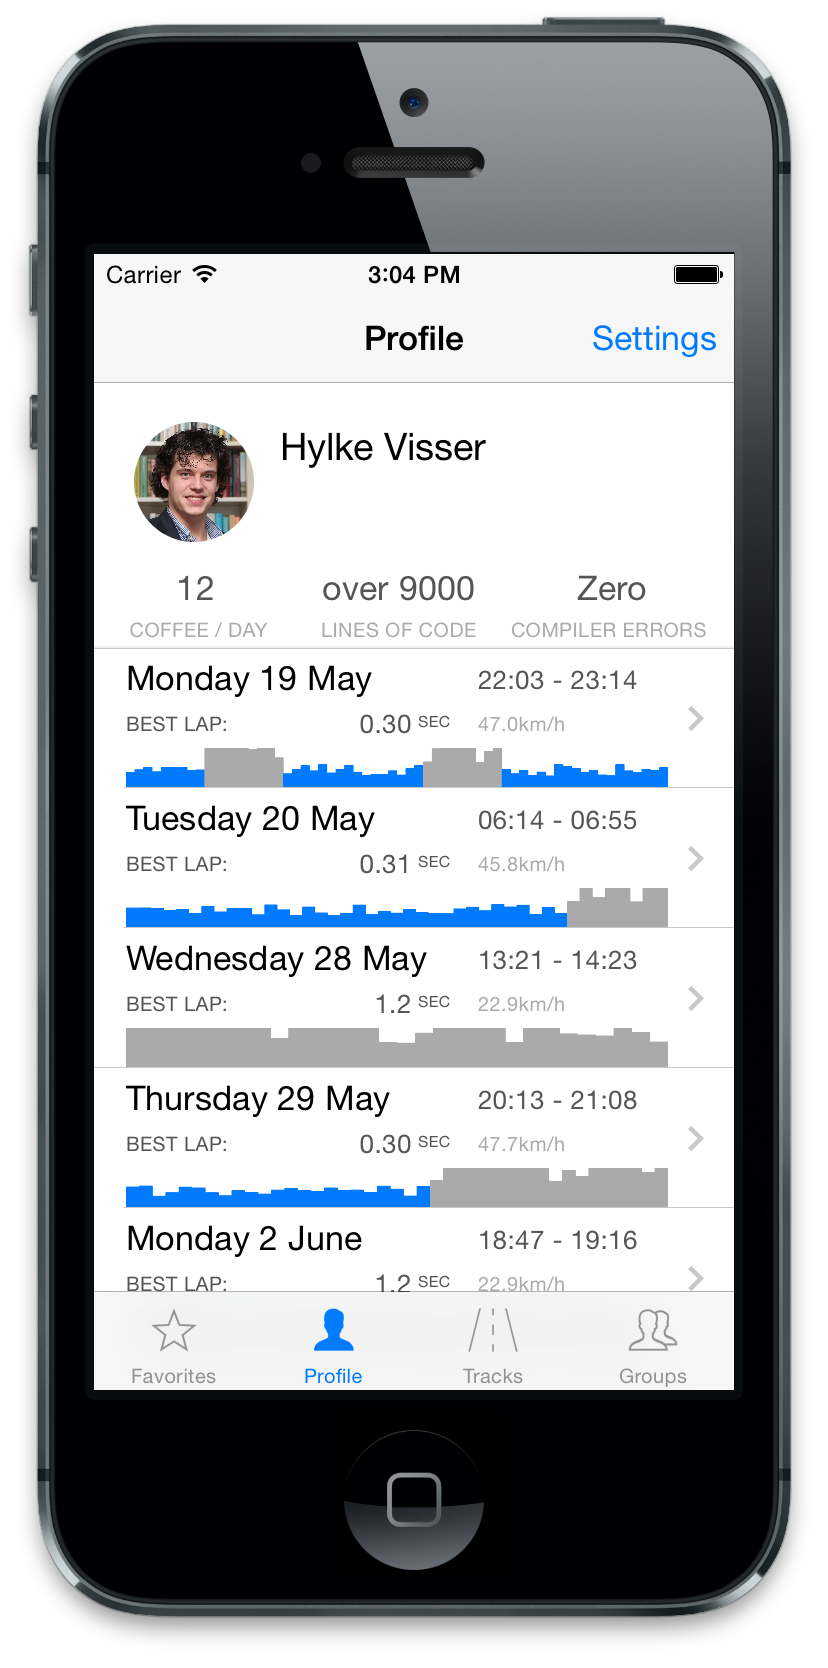
\includegraphics[width=4cm]{style/images/screenshots/I-03-Home}
  \end{center}
  \caption{Het profielscherm met het sessieoverzicht}
  \label{fig:profiel-scherm}
\end{wrapfigure}

Om ervoor te zorgen dat de applicatie nog steeds snel aanvoelt, worden de grafiekjes die waarschijnlijk niet meer zullen veranderen, omgezet in afbeeldingen en gecached, zodat ze niet telkens opnieuw getekend hoeven te worden.
